\documentclass[xcolor=svgnames]{beamer}\usepackage[]{graphicx}\usepackage[]{color}
%% maxwidth is the original width if it is less than linewidth
%% otherwise use linewidth (to make sure the graphics do not exceed the margin)
\makeatletter
\def\maxwidth{ %
  \ifdim\Gin@nat@width>\linewidth
    \linewidth
  \else
    \Gin@nat@width
  \fi
}
\makeatother

\definecolor{fgcolor}{rgb}{0.345, 0.345, 0.345}
\newcommand{\hlnum}[1]{\textcolor[rgb]{0.686,0.059,0.569}{#1}}%
\newcommand{\hlstr}[1]{\textcolor[rgb]{0.192,0.494,0.8}{#1}}%
\newcommand{\hlcom}[1]{\textcolor[rgb]{0.678,0.584,0.686}{\textit{#1}}}%
\newcommand{\hlopt}[1]{\textcolor[rgb]{0,0,0}{#1}}%
\newcommand{\hlstd}[1]{\textcolor[rgb]{0.345,0.345,0.345}{#1}}%
\newcommand{\hlkwa}[1]{\textcolor[rgb]{0.161,0.373,0.58}{\textbf{#1}}}%
\newcommand{\hlkwb}[1]{\textcolor[rgb]{0.69,0.353,0.396}{#1}}%
\newcommand{\hlkwc}[1]{\textcolor[rgb]{0.333,0.667,0.333}{#1}}%
\newcommand{\hlkwd}[1]{\textcolor[rgb]{0.737,0.353,0.396}{\textbf{#1}}}%

\usepackage{framed}
\makeatletter
\newenvironment{kframe}{%
 \def\at@end@of@kframe{}%
 \ifinner\ifhmode%
  \def\at@end@of@kframe{\end{minipage}}%
  \begin{minipage}{\columnwidth}%
 \fi\fi%
 \def\FrameCommand##1{\hskip\@totalleftmargin \hskip-\fboxsep
 \colorbox{shadecolor}{##1}\hskip-\fboxsep
     % There is no \\@totalrightmargin, so:
     \hskip-\linewidth \hskip-\@totalleftmargin \hskip\columnwidth}%
 \MakeFramed {\advance\hsize-\width
   \@totalleftmargin\z@ \linewidth\hsize
   \@setminipage}}%
 {\par\unskip\endMakeFramed%
 \at@end@of@kframe}
\makeatother

\definecolor{shadecolor}{rgb}{.97, .97, .97}
\definecolor{messagecolor}{rgb}{0, 0, 0}
\definecolor{warningcolor}{rgb}{1, 0, 1}
\definecolor{errorcolor}{rgb}{1, 0, 0}
\newenvironment{knitrout}{}{} % an empty environment to be redefined in TeX

\usepackage{alltt}
\usetheme{Boadilla}
\usecolortheme[named=SeaGreen]{structure}
\usepackage{graphicx}
\usepackage{breqn}
\usepackage{xcolor}
\usepackage{booktabs}
\usepackage{verbatim}
\usepackage{tikz}
\usepackage{lmodern}
\usetikzlibrary{shadows,arrows,positioning}
\definecolor{links}{HTML}{2A1B81}
\hypersetup{colorlinks,linkcolor=links,urlcolor=links}
\usepackage{pgfpages}

\newcommand{\Bigtxt}[1]{\textbf{\textit{#1}}}
\IfFileExists{upquote.sty}{\usepackage{upquote}}{}
\begin{document}

\title[SWMP organizing]{Processing and organizing SWMP time series for analysis}

\author[M. Beck, T. O'Brien]{Marcus W. Beck\inst{1} \and Todd D. O'Brien\inst{2}}

\date{}

\institute[]{\inst{1} ORISE, USEPA NHEERL Gulf Ecology Division\\ Email: \href{mailto:beck.marcus@epa.gov}{beck.marcus@epa.gov} \and \inst{2} NOAA/NMFS COPEPOD Project\\ Email: \href{todd.obrien@noaa.gov}{todd.obrien@noaa.gov}}

% knitr setup


% load SWMPr from local


%%%%%%
\begin{frame}
\vspace{0.3in}
\centerline{
\begin{tikzpicture}
  \node[drop shadow={shadow xshift=0ex,shadow yshift=0ex},fill=white,draw] at (0,0) {
\includegraphics[width=0.9\textwidth]{bg_main.jpg}};
\end{tikzpicture}}
\titlepage
\end{frame}

%%%%%%
\begin{frame}{Objectives and agenda}
\begin{itemize}
\onslide<+->
\item Objectives \\~\\
\begin{itemize}
\item How can SWMP data quality be evaluated and handled? \\~\\
\item How can data be selected and removed to facilitate analysis? \\~\\
\item What are some ways that date are combined and why would this be done? \\~\\
\end{itemize}
\onslide<+->
\item Agenda \\~\\
\begin{itemize}
\item Review of import and handling QAQC flags\\~\\
\item Appropriate use of data subsets \\~\\
\item Combining data for comparisons \\~\\
\end{itemize}
\end{itemize}
\end{frame}

%%%%%%
\begin{frame}{Interactive portion}
You can follow along in this module: \\~\\
\begin{itemize}
\item dataset2 \\~\\
\item script2 \\~\\
\end{itemize}
\Large
\centerline{\emph{Interactive!}}
\end{frame}

%%%%%%
\begin{frame}{Retrieve SWMP data}
We learned how to import SWMP data in the previous session \\~\\
To review, the easiest approach is to download the data outside of R, then import using the `import_local' function \\~\\
Be sure that you use only the \href{http://cdmo.baruch.sc.edu/aqs/zips.cfm}{zip downloads} feature from CDMO - the `import_local' functions works best with these data \\~\\
\centerline{
\includegraphics[width = 0.8\textwidth]{adv_query.png}}
\end{frame}

%%%%%%
\begin{frame}[t]{Retrieve SWMP data}
We have provided data for use with the workshop\\~\\
For future access, it may be best to download all the data possible for a reserve to avoid repeated requests to the server and to centralize the location from which the data are imported into R \\~\\
\centerline{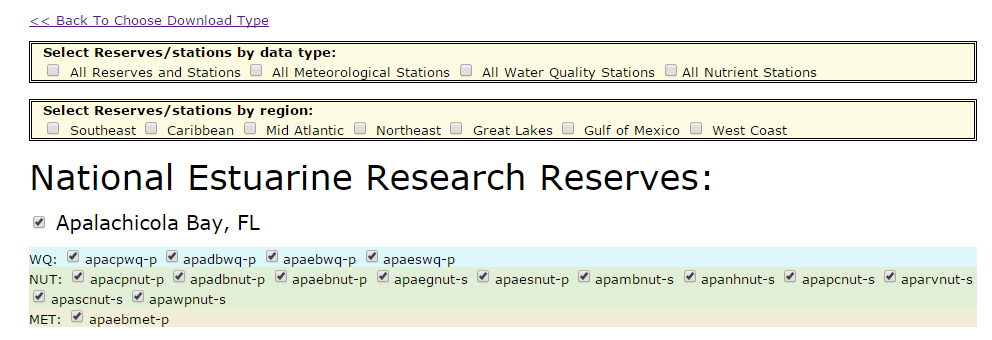
\includegraphics[width = \textwidth]{zip_eda.png}}
\end{frame}

%%%%%%
\begin{frame}[t]{Retrieve SWMP data}
It may be best to download all the data possible for a reserve to avoid repeated requests to the server and to centralize the location from which the data are imported into R \\~\\
\centerline{
\includegraphics[width = 0.5\textwidth]{zip_eda2.png}}
Here we've made a request for all stations at Apalachicola Bay (water quality, nutrients, weather) and all available years (1995--2014) \\~\\
This request will take several minutes to be delivered to your email - the files in `dataset2' are an abbreviate version of these data for this training module
\end{frame}

%%%%%%
\begin{frame}[containsverbatim]{Retrieve SWMP data}
Let's import some data for Apalachicola Bay

\begin{knitrout}\scriptsize
\definecolor{shadecolor}{rgb}{0.969, 0.969, 0.969}\color{fgcolor}\begin{kframe}
\begin{alltt}
\hlcom{# reload the SWMPr package if you started a new session}
\hlkwd{library}\hlstd{(SWMPr)}

\hlcom{# import data}
\hlcom{# change this path for the flash drive}
\hlstd{path} \hlkwb{<-} \hlstr{'C:/data/dataset2'}
\hlstd{wq_dat} \hlkwb{<-} \hlkwd{import_local}\hlstd{(path,} \hlstr{'apacpwq'}\hlstd{)}
\hlstd{nut_dat} \hlkwb{<-} \hlkwd{import_local}\hlstd{(path,} \hlstr{'apacpnut'}\hlstd{)}
\hlstd{met_dat} \hlkwb{<-} \hlkwd{import_local}\hlstd{(path,} \hlstr{'apaebmet'}\hlstd{)}
\end{alltt}
\end{kframe}
\end{knitrout}
We've just imported data from 2011--2014 for three stations (apacpwq, apacpnut, apaebmet) and saved them in our workspace as three separate objects (wq\_dat, nut\_dat, met\_dat)
\end{frame}

%%%%%%
\begin{frame}[containsverbatim]{Retrieve SWMP data}
But don't take my word for it, take a look at the data!
\begin{knitrout}\scriptsize
\definecolor{shadecolor}{rgb}{0.969, 0.969, 0.969}\color{fgcolor}\begin{kframe}
\begin{alltt}
\hlcom{# what are the dimenions of the water quality data?}
\hlkwd{dim}\hlstd{(wq_dat)}
\end{alltt}
\begin{verbatim}
## [1] 132035     25
\end{verbatim}
\begin{alltt}
\hlcom{# what are the dimenions of the nutrient data?}
\hlkwd{dim}\hlstd{(nut_dat)}
\end{alltt}
\begin{verbatim}
## [1] 48 13
\end{verbatim}
\begin{alltt}
\hlcom{# what are the dimenions of the weather data?}
\hlkwd{dim}\hlstd{(met_dat)}
\end{alltt}
\begin{verbatim}
## [1] 133548     23
\end{verbatim}
\end{kframe}
\end{knitrout}
\end{frame}

%%%%%%
\begin{frame}[containsverbatim,shrink]{Retrieve SWMP data}
View the first six rows
\begin{knitrout}\scriptsize
\definecolor{shadecolor}{rgb}{0.969, 0.969, 0.969}\color{fgcolor}\begin{kframe}
\begin{alltt}
\hlcom{# View the first six rows of the met data}
\hlkwd{head}\hlstd{(met_dat)}
\end{alltt}
\begin{verbatim}
##         datetimestamp atemp f_atemp rh f_rh   bp f_bp wspd f_wspd maxwspd
## 1 2011-01-01 00:00:00    15    <0>  94 <0>  1019 <0>     3   <0>        3
## 2 2011-01-01 00:15:00    15    <0>  95 <0>  1019 <0>     3   <0>        4
## 3 2011-01-01 00:30:00    15    <0>  95 <0>  1019 <0>     3   <0>        4
## 4 2011-01-01 00:45:00    15    <0>  95 <0>  1019 <0>     3   <0>        4
## 5 2011-01-01 01:00:00    15    <0>  95 <0>  1018 <0>     3   <0>        4
## 6 2011-01-01 01:15:00    15    <0>  95 <0>  1018 <0>     4   <0>        5
##   f_maxwspd wdir f_wdir sdwdir f_sdwdir totpar  f_totpar totprcp f_totprcp
## 1      <0>   145   <0>       8     <0>     0.8 <1> (CSM)       0      <0> 
## 2      <0>   146   <0>       7     <0>     0.8 <1> (CSM)       0      <0> 
## 3      <0>   139   <0>       7     <0>     0.8 <1> (CSM)       0      <0> 
## 4      <0>   140   <0>       7     <0>     0.8 <1> (CSM)       0      <0> 
## 5      <0>   144   <0>       6     <0>     0.8 <1> (CSM)       0      <0> 
## 6      <0>   141   <0>       7     <0>     0.8 <1> (CSM)       0      <0> 
##   cumprcp f_cumprcp totsorad f_totsorad
## 1       0      <0>        NA      <-1> 
## 2       0      <0>        NA      <-1> 
## 3       0      <0>        NA      <-1> 
## 4       0      <0>        NA      <-1> 
## 5       0      <0>        NA      <-1> 
## 6       0      <0>        NA      <-1>
\end{verbatim}
\end{kframe}
\end{knitrout}
\end{frame}

%%%%%%
\begin{frame}[containsverbatim,shrink]{Retrieve SWMP data}
View the last six rows
\begin{knitrout}\scriptsize
\definecolor{shadecolor}{rgb}{0.969, 0.969, 0.969}\color{fgcolor}\begin{kframe}
\begin{alltt}
\hlcom{# View the last six rows of the met data}
\hlkwd{tail}\hlstd{(met_dat)}
\end{alltt}
\begin{verbatim}
##              datetimestamp atemp f_atemp rh f_rh   bp f_bp wspd f_wspd maxwspd
## 133543 2014-10-23 01:30:00    14    <0>  72 <0>  1017 <0>     3   <0>        5
## 133544 2014-10-23 01:45:00    14    <0>  72 <0>  1016 <0>     3   <0>        5
## 133545 2014-10-23 02:00:00    14    <0>  74 <0>  1016 <0>     3   <0>        4
## 133546 2014-10-23 02:15:00    14    <0>  74 <0>  1016 <0>     3   <0>        4
## 133547 2014-10-23 02:30:00    14    <0>  75 <0>  1016 <0>     3   <0>        4
## 133548 2014-10-23 02:45:00    14    <0>  76 <0>  1016 <0>     2   <0>        4
##        f_maxwspd wdir f_wdir sdwdir f_sdwdir totpar f_totpar totprcp f_totprcp
## 133543      <0>    33   <0>       9     <0>       0     <0>        0      <0> 
## 133544      <0>    34   <0>      11     <0>       0     <0>        0      <0> 
## 133545      <0>    36   <0>      10     <0>       0     <0>        0      <0> 
## 133546      <0>    43   <0>      11     <0>       0     <0>        0      <0> 
## 133547      <0>    41   <0>      10     <0>       0     <0>        0      <0> 
## 133548      <0>    42   <0>      10     <0>       0     <0>        0      <0> 
##        cumprcp f_cumprcp totsorad f_totsorad
## 133543      NA     <-2>        NA      <-1> 
## 133544      NA     <-2>        NA      <-1> 
## 133545      NA     <-2>        NA      <-1> 
## 133546      NA     <-2>        NA      <-1> 
## 133547      NA     <-2>        NA      <-1> 
## 133548      NA     <-2>        NA      <-1>
\end{verbatim}
\end{kframe}
\end{knitrout}
\end{frame}

%%%%%%
\begin{frame}[containsverbatim,shrink]{Retrieve SWMP data}
We'll first work with the water quality records\\~\\
What class is the data?
\begin{knitrout}\scriptsize
\definecolor{shadecolor}{rgb}{0.969, 0.969, 0.969}\color{fgcolor}\begin{kframe}
\begin{alltt}
\hlcom{# class of the data}
\hlkwd{class}\hlstd{(met_dat)}
\end{alltt}
\begin{verbatim}
## [1] "swmpr"      "data.frame"
\end{verbatim}
\end{kframe}
\end{knitrout}
This tells us that the data are two different classes - `swmpr' and `data.frame'\\~\\
The class of an object is important because it defines the types of methods (i.e., functions) that apply\\~\\
For example, `head' and `tail' functions work for a `data.frame'
\end{frame}

%%%%%%
\begin{frame}[containsverbatim,shrink]{Retrieve SWMP data}
The swmpr object class was developed to make your life easier working with SWMP data\\~\\
The \href{https://github.com/fawda123/SWMPr}{online documentation} describes the functions that work with the swmpr object class, also...
\begin{knitrout}\scriptsize
\definecolor{shadecolor}{rgb}{0.969, 0.969, 0.969}\color{fgcolor}\begin{kframe}
\begin{alltt}
\hlcom{# what functions/methods work with swmpr objects?}
\hlkwd{methods}\hlstd{(}\hlkwc{class} \hlstd{=} \hlstr{'swmpr'}\hlstd{)}
\end{alltt}
\begin{verbatim}
##  [1] aggregate.swmpr comb.swmpr      decomp.swmpr    hist.swmpr     
##  [5] lines.swmpr     na.approx.swmpr plot.swmpr      qaqc.swmpr     
##  [9] qaqcchk.swmpr   setstep.swmpr   smoother.swmpr  subset.swmpr
\end{verbatim}
\end{kframe}
\end{knitrout}
Documentation of each function can be viewed as follows (although currently not complete):
\begin{knitrout}\scriptsize
\definecolor{shadecolor}{rgb}{0.969, 0.969, 0.969}\color{fgcolor}\begin{kframe}
\begin{alltt}
\hlcom{# see help for a swmpr function}
\hlopt{?}\hlstd{aggregate.swmpr}

\hlcom{# or...}
\hlkwd{help}\hlstd{(}\hlstr{'aggregate.swmpr'}\hlstd{)}
\end{alltt}
\end{kframe}
\end{knitrout}
\end{frame}

%%%%%%
\begin{frame}[containsverbatim,shrink]{Retrieve SWMP data}
A side note about R syntax... the convention `function.class' means that a function applies to a specific class \\~\\
The `function' is generic, whereas the `function.class' is a method for a class that applies to the generic
\begin{knitrout}\scriptsize
\definecolor{shadecolor}{rgb}{0.969, 0.969, 0.969}\color{fgcolor}\begin{kframe}
\begin{alltt}
\hlcom{# view the methods that apply to the generic aggregate}
\hlkwd{methods}\hlstd{(}\hlstr{'aggregate'}\hlstd{)}
\end{alltt}
\begin{verbatim}
## [1] aggregate.data.frame aggregate.default*   aggregate.formula*  
## [4] aggregate.swmpr      aggregate.ts         aggregate.zoo*      
## 
##    Non-visible functions are asterisked
\end{verbatim}
\end{kframe}
\end{knitrout}
A function with a class method can be executed using shorthand...
\begin{knitrout}\scriptsize
\definecolor{shadecolor}{rgb}{0.969, 0.969, 0.969}\color{fgcolor}\begin{kframe}
\begin{alltt}
\hlcom{# shorthand for executing aggregate on a swmpr object}
\hlkwd{aggregate}\hlstd{(met_dat,} \hlkwc{by} \hlstd{=} \hlstr{'quarters'}\hlstd{)}

\hlcom{# long also works}
\hlkwd{aggregate.swmpr}\hlstd{(met_dat,} \hlkwc{by} \hlstd{=} \hlstr{'quarters'}\hlstd{)}
\end{alltt}
\end{kframe}
\end{knitrout}
\end{frame}

%%%%%
\begin{frame}[containsverbatim,shrink]{Retrieve SWMP data}
A useful feature of R is that a class will have both \Bigtxt{data} and \Bigtxt{attributes}\\~\\
For the swmpr class, the \Bigtxt{data} are the raw swmpr data as a data.frame \\~\\
The \Bigtxt{attributes} are a list of metadata for the imported data
\begin{knitrout}\scriptsize
\definecolor{shadecolor}{rgb}{0.969, 0.969, 0.969}\color{fgcolor}\begin{kframe}
\begin{alltt}
\hlcom{# what attributes are available for a swmpr object}
\hlkwd{names}\hlstd{(}\hlkwd{attributes}\hlstd{(met_dat))}
\end{alltt}
\begin{verbatim}
## [1] "names"       "row.names"   "class"       "station"     "parameters" 
## [6] "qaqc_cols"   "date_rng"    "timezone"    "stamp_class"
\end{verbatim}
\begin{alltt}
\hlcom{# view the parameters}
\hlkwd{attr}\hlstd{(met_dat,} \hlstr{'parameters'}\hlstd{)}
\end{alltt}
\begin{verbatim}
##  [1] "atemp"    "rh"       "bp"       "wspd"     "maxwspd"  "wdir"    
##  [7] "sdwdir"   "totpar"   "totprcp"  "cumprcp"  "totsorad"
\end{verbatim}
\end{kframe}
\end{knitrout}
\end{frame}

%%%%%
\begin{frame}[containsverbatim]{Retrieve SWMP data}
You can also view all the attributes as follows:
\begin{knitrout}\scriptsize
\definecolor{shadecolor}{rgb}{0.969, 0.969, 0.969}\color{fgcolor}\begin{kframe}
\begin{alltt}
\hlcom{# view all attributes}
\hlkwd{attributes}\hlstd{(met_dat)}
\end{alltt}
\end{kframe}
\end{knitrout}
This is not recommended since they are quite long, e.g., an attribute of the `data.frame' class is the row names (132035 rows for`wq\_dat') \\~\\
Individual attributes are useful for getting a feel for the dataset - what is the date range? what parameters are included? are QAQC columns present? \\~\\
However, the intended use of attributes is behind the scenes with swmpr functions - they will be used to process the data and updated automatically
\end{frame}

%%%%%%
\begin{frame}[containsverbatim]{Retrieve SWMP data}
A summary of the swmpr object class:\\~\\
\begin{itemize}
\item Throughout `SWMPr' refers to the \Bigtxt{package}, `swmpr' refers to the object \Bigtxt{class}
\item \Bigtxt{Methods} aka functions in the SWMPr package are specific for swmpr objects - see the help documentation (`?aggregate.swmpr')
\item The swmpr object has both \Bigtxt{data} and \Bigtxt{attributes} - the data are in the `data.frame' format, the attributes are in a `list'\\~\\
\end{itemize}
These are basic concepts that are fundamental to how the R language works -- you should have a general understanding of their meaning
\end{frame}

%%%%%%
\begin{frame}[containsverbatim,shrink]{Organize SWMP data}
Now that we have a feel for the data, what needs to be done before we can start analyzing the information? \\~\\
Last module: \\~\\
\begin{itemize}
\item How do we handle QAQC data or `bad' observations?
\item How do we deal with data we don't want?  
\item How do we combine data for comparison?
\item How do we handle issues inherent with time series? \\~\\
\end{itemize}
Several of these problems are context-dependent - driven by the question or analysis \\~\\
Others are common to any analysis...
\end{frame}

%%%%%%
\begin{frame}[containsverbatim]{Organize SWMP data}
Perhaps the first organizational tool you want to use is `qaqc.swmpr'\\~\\
This function does two things:\\~\\
\begin{itemize}
\item Remove observations with a specified QAQC flag value
\item Remove QAQC columns \\~\\
\end{itemize}
\centerline{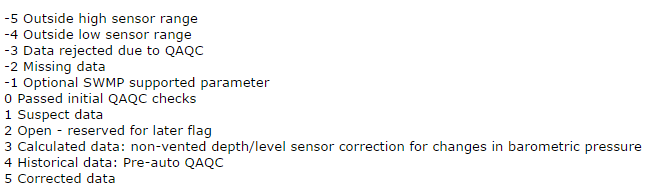
\includegraphics[width = 0.8\textwidth]{qaqc_flags.png}}
\end{frame}

%%%%%%
\begin{frame}[containsverbatim,shrink]{Retrieve SWMP data}
Remember, each parameter has a QAQC column preceded by `f_'
\begin{knitrout}\scriptsize
\definecolor{shadecolor}{rgb}{0.969, 0.969, 0.969}\color{fgcolor}\begin{kframe}
\begin{alltt}
\hlcom{# View the first six rows of the met data}
\hlkwd{head}\hlstd{(met_dat)}
\end{alltt}
\begin{verbatim}
##         datetimestamp atemp f_atemp rh f_rh   bp f_bp wspd f_wspd maxwspd
## 1 2011-01-01 00:00:00    15    <0>  94 <0>  1019 <0>     3   <0>        3
## 2 2011-01-01 00:15:00    15    <0>  95 <0>  1019 <0>     3   <0>        4
## 3 2011-01-01 00:30:00    15    <0>  95 <0>  1019 <0>     3   <0>        4
## 4 2011-01-01 00:45:00    15    <0>  95 <0>  1019 <0>     3   <0>        4
## 5 2011-01-01 01:00:00    15    <0>  95 <0>  1018 <0>     3   <0>        4
## 6 2011-01-01 01:15:00    15    <0>  95 <0>  1018 <0>     4   <0>        5
##   f_maxwspd wdir f_wdir sdwdir f_sdwdir totpar  f_totpar totprcp f_totprcp
## 1      <0>   145   <0>       8     <0>     0.8 <1> (CSM)       0      <0> 
## 2      <0>   146   <0>       7     <0>     0.8 <1> (CSM)       0      <0> 
## 3      <0>   139   <0>       7     <0>     0.8 <1> (CSM)       0      <0> 
## 4      <0>   140   <0>       7     <0>     0.8 <1> (CSM)       0      <0> 
## 5      <0>   144   <0>       6     <0>     0.8 <1> (CSM)       0      <0> 
## 6      <0>   141   <0>       7     <0>     0.8 <1> (CSM)       0      <0> 
##   cumprcp f_cumprcp totsorad f_totsorad
## 1       0      <0>        NA      <-1> 
## 2       0      <0>        NA      <-1> 
## 3       0      <0>        NA      <-1> 
## 4       0      <0>        NA      <-1> 
## 5       0      <0>        NA      <-1> 
## 6       0      <0>        NA      <-1>
\end{verbatim}
\end{kframe}
\end{knitrout}
\end{frame}

%%%%%%
\begin{frame}[containsverbatim]{Organize SWMP data}
You will have to decide which \href{http://cdmo.baruch.sc.edu/data/qaqc.cfm}{values} to keep - be conservative and only keep those that passed QAQC or keep all the data \\~\\
To help you decide, it may be useful to get an idea of the distribution of QAQC flags in the data, use `qaqcchk'
\begin{knitrout}\scriptsize
\definecolor{shadecolor}{rgb}{0.969, 0.969, 0.969}\color{fgcolor}\begin{kframe}
\begin{alltt}
\hlcom{# use qaqcchk to view distribution of qaqc flags}
\hlstd{myqaqc} \hlkwb{<-} \hlkwd{qaqcchk}\hlstd{(met_dat)}
\end{alltt}
\end{kframe}
\end{knitrout}
This function returns a data.frame\\~\\
\begin{itemize}
\item The first column shows all the QAQC codes in the data
\item The remaining columns show the counts for each parameter of the observations assigned to each QAQC code
\end{itemize}
\end{frame}

%%%%%%
\begin{frame}[containsverbatim]{Organize SWMP data}
\begin{knitrout}\scriptsize
\definecolor{shadecolor}{rgb}{0.969, 0.969, 0.969}\color{fgcolor}\begin{kframe}
\begin{alltt}
\hlcom{# a subset of results from the qaqcchk function}
\hlkwd{head}\hlstd{(myqaqc)}
\end{alltt}
\begin{verbatim}
##              piece f_atemp f_bp f_cumprcp f_maxwspd f_rh f_sdwdir f_totpar
## 1       <-2> [GPD]       2    2         2         2    2        2        2
## 2       <-3> [GMT]       5   13        70        16    5       16       18
## 3       <-3> [GPD]      15   16        16        16   15       16       16
## 4       <-3> [GPR]      14   14        14        14   14       14       13
## 5       <-3> [SMT]       2   NA       121         3    2        3        2
## 6 <-3> [SQR] (CSM)       3   NA        NA        NA    3       NA     4023
##   f_totprcp f_totsorad f_wdir f_wspd
## 1         2         NA      2      2
## 2        13         NA     16     16
## 3        16         NA     16     16
## 4        14         NA     14     14
## 5        14         NA      3      3
## 6        NA         NA     NA     NA
\end{verbatim}
\begin{alltt}
\hlcom{# or view all in a separate window}
\hlkwd{View}\hlstd{(myqaqc)}
\end{alltt}
\end{kframe}
\end{knitrout}
\href{http://cdmo.baruch.sc.edu/data/qaqc.cfm}{Link} to QAQC codes
\end{frame}

%%%%%%
\begin{frame}[containsverbatim]{Organize SWMP data}
A plot of the data may also be useful to view QAQC flags, but this is tedious \\~\\
Here's an example for the `totpar' variable
\begin{knitrout}\scriptsize
\definecolor{shadecolor}{rgb}{0.969, 0.969, 0.969}\color{fgcolor}\begin{kframe}
\begin{alltt}
\hlcom{# select values that did not pass qaqc}
\hlstd{nopass} \hlkwb{<-} \hlkwd{grep}\hlstd{(}\hlstr{'0'}\hlstd{, met_dat}\hlopt{$}\hlstd{f_totpar,} \hlkwc{invert} \hlstd{= T)}
\hlstd{nopass} \hlkwb{<-} \hlstd{met_dat[nopass, ]}

\hlcom{# plot totpar from met_dat}
\hlkwd{plot}\hlstd{(totpar} \hlopt{~} \hlstd{datetimestamp, met_dat,} \hlkwc{type} \hlstd{=} \hlstr{'l'}\hlstd{)}

\hlcom{# add  points that did not pass qaqc}
\hlkwd{points}\hlstd{(nopass}\hlopt{$}\hlstd{datetimestamp, nopass}\hlopt{$}\hlstd{totpar,} \hlkwc{col} \hlstd{=} \hlstr{'red'}\hlstd{)}
\end{alltt}
\end{kframe}
\end{knitrout}
\end{frame}

%%%%%%
\begin{frame}[containsverbatim]{Organize SWMP data}
Observations in red are those that did not pass QAQC checks - some are obvious, others are not
\begin{knitrout}\scriptsize
\definecolor{shadecolor}{rgb}{0.969, 0.969, 0.969}\color{fgcolor}

{\centering 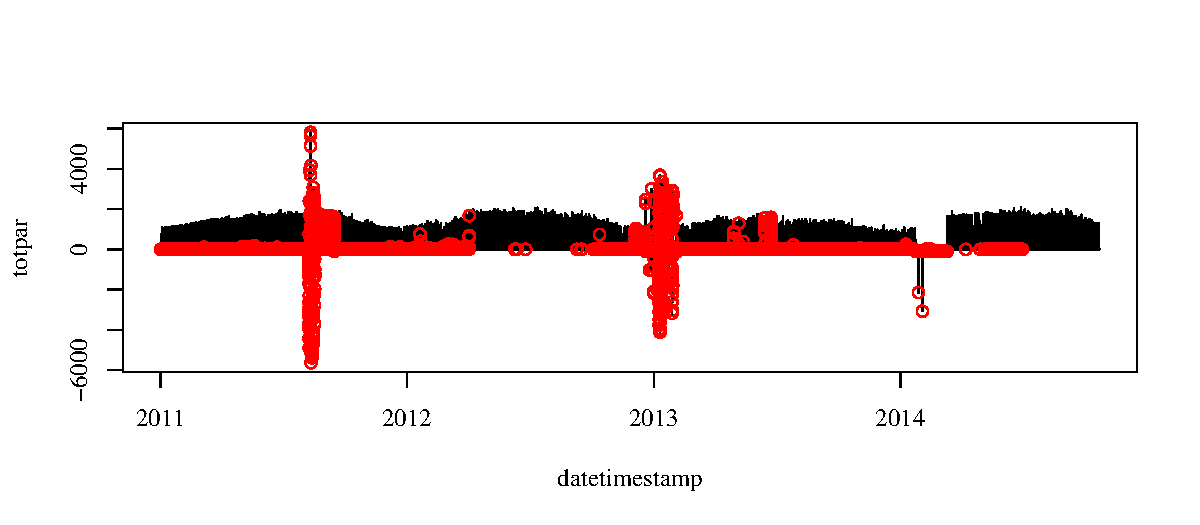
\includegraphics[width=\maxwidth]{figure/qaqc_ex} 

}



\end{knitrout}
Does this plot make sense??
\end{frame}

%%%%%%
\begin{frame}[containsverbatim]{Organize SWMP data}
You should have an idea of how you want to handle QAQC values after viewing the output from qaqcchk or plotting - or you already knew \\~\\
Next, use the `qaqc' function...
\begin{knitrout}\scriptsize
\definecolor{shadecolor}{rgb}{0.969, 0.969, 0.969}\color{fgcolor}\begin{kframe}
\begin{alltt}
\hlcom{# filter observations by qaqc flags, remove qaqc columns}
\hlstd{met_qaqc} \hlkwb{<-} \hlkwd{qaqc}\hlstd{(met_dat)}
\end{alltt}
\end{kframe}
\end{knitrout}
The default behavior for this function is to keep only observations with a `0' QAQC flag - data that passed initial checks\\~\\
See the help documentation for the function
\begin{knitrout}\scriptsize
\definecolor{shadecolor}{rgb}{0.969, 0.969, 0.969}\color{fgcolor}\begin{kframe}
\begin{alltt}
\hlcom{# view help file}
\hlopt{?}\hlstd{qaqc}
\end{alltt}
\end{kframe}
\end{knitrout}
\end{frame}

%%%%%%
\begin{frame}[containsverbatim]{Organize SWMP data}
View the data after keeping only values that passed QAQC (`0' flag)
\begin{knitrout}\scriptsize
\definecolor{shadecolor}{rgb}{0.969, 0.969, 0.969}\color{fgcolor}\begin{kframe}
\begin{alltt}
\hlcom{# data after qaqc processing}
\hlkwd{head}\hlstd{(met_qaqc)}
\end{alltt}
\begin{verbatim}
##         datetimestamp atemp rh   bp wspd maxwspd wdir sdwdir totpar totprcp
## 1 2011-01-01 00:00:00    15 94 1019    3       3  145      8     NA       0
## 2 2011-01-01 00:15:00    15 95 1019    3       4  146      7     NA       0
## 3 2011-01-01 00:30:00    15 95 1019    3       4  139      7     NA       0
## 4 2011-01-01 00:45:00    15 95 1019    3       4  140      7     NA       0
## 5 2011-01-01 01:00:00    15 95 1018    3       4  144      6     NA       0
## 6 2011-01-01 01:15:00    15 95 1018    4       5  141      7     NA       0
##   cumprcp totsorad
## 1       0       NA
## 2       0       NA
## 3       0       NA
## 4       0       NA
## 5       0       NA
## 6       0       NA
\end{verbatim}
\end{kframe}
\end{knitrout}
\end{frame}

%%%%%%
\begin{frame}[containsverbatim]{Organize SWMP data}
What if we want to keep all the values, regardless of flag?
\begin{knitrout}\scriptsize
\definecolor{shadecolor}{rgb}{0.969, 0.969, 0.969}\color{fgcolor}\begin{kframe}
\begin{alltt}
\hlcom{# keep all values}
\hlstd{met_qaqc} \hlkwb{<-} \hlkwd{qaqc}\hlstd{(met_dat,} \hlkwc{qaqc_keep} \hlstd{=} \hlkwa{NULL}\hlstd{)}

\hlkwd{head}\hlstd{(met_qaqc)} \hlcom{# note the totpar column compared to the last example}
\end{alltt}
\begin{verbatim}
##         datetimestamp atemp rh   bp wspd maxwspd wdir sdwdir totpar totprcp
## 1 2011-01-01 00:00:00    15 94 1019    3       3  145      8    0.8       0
## 2 2011-01-01 00:15:00    15 95 1019    3       4  146      7    0.8       0
## 3 2011-01-01 00:30:00    15 95 1019    3       4  139      7    0.8       0
## 4 2011-01-01 00:45:00    15 95 1019    3       4  140      7    0.8       0
## 5 2011-01-01 01:00:00    15 95 1018    3       4  144      6    0.8       0
## 6 2011-01-01 01:15:00    15 95 1018    4       5  141      7    0.8       0
##   cumprcp totsorad
## 1       0       NA
## 2       0       NA
## 3       0       NA
## 4       0       NA
## 5       0       NA
## 6       0       NA
\end{verbatim}
\end{kframe}
\end{knitrout}
\end{frame}

%%%%%%
\begin{frame}[containsverbatim]{Organize SWMP data}
If you're not convinced, try removing only the `0' flag
\begin{knitrout}\scriptsize
\definecolor{shadecolor}{rgb}{0.969, 0.969, 0.969}\color{fgcolor}\begin{kframe}
\begin{alltt}
\hlcom{# keep all values}
\hlstd{to_keep} \hlkwb{<-} \hlkwd{c}\hlstd{(}\hlopt{-}\hlnum{5}\hlstd{,} \hlopt{-}\hlnum{4}\hlstd{,} \hlopt{-}\hlnum{3}\hlstd{,} \hlopt{-}\hlnum{2}\hlstd{,} \hlopt{-}\hlnum{1}\hlstd{,} \hlnum{1}\hlstd{,} \hlnum{2}\hlstd{,} \hlnum{3}\hlstd{,} \hlnum{4}\hlstd{,} \hlnum{5}\hlstd{)}
\hlstd{met_qaqc} \hlkwb{<-} \hlkwd{qaqc}\hlstd{(met_dat,} \hlkwc{qaqc_keep} \hlstd{= to_keep)}

\hlcom{# does this result make sense??}
\hlkwd{head}\hlstd{(met_qaqc)}
\end{alltt}
\begin{verbatim}
##         datetimestamp atemp rh bp wspd maxwspd wdir sdwdir totpar totprcp
## 1 2011-01-01 00:00:00    NA NA NA   NA      NA   NA     NA    0.8      NA
## 2 2011-01-01 00:15:00    NA NA NA   NA      NA   NA     NA    0.8      NA
## 3 2011-01-01 00:30:00    NA NA NA   NA      NA   NA     NA    0.8      NA
## 4 2011-01-01 00:45:00    NA NA NA   NA      NA   NA     NA    0.8      NA
## 5 2011-01-01 01:00:00    NA NA NA   NA      NA   NA     NA    0.8      NA
## 6 2011-01-01 01:15:00    NA NA NA   NA      NA   NA     NA    0.8      NA
##   cumprcp totsorad
## 1      NA       NA
## 2      NA       NA
## 3      NA       NA
## 4      NA       NA
## 5      NA       NA
## 6      NA       NA
\end{verbatim}
\end{kframe}
\end{knitrout}
\end{frame}

%%%%%%
\begin{frame}[containsverbatim]{Organize SWMP data}
We'll continue by using values that passed the QAQC checks
\begin{knitrout}\scriptsize
\definecolor{shadecolor}{rgb}{0.969, 0.969, 0.969}\color{fgcolor}\begin{kframe}
\begin{alltt}
\hlcom{# continue with qaqc processed data}

\hlcom{# water quality}
\hlcom{# note the column number before/after qaqc processing}
\hlkwd{dim}\hlstd{(wq_dat)}
\end{alltt}
\begin{verbatim}
## [1] 132035     25
\end{verbatim}
\begin{alltt}
\hlstd{wq_dat} \hlkwb{<-} \hlkwd{qaqc}\hlstd{(wq_dat)}
\hlkwd{dim}\hlstd{(wq_dat)}
\end{alltt}
\begin{verbatim}
## [1] 132035     13
\end{verbatim}
\begin{alltt}
\hlcom{# nutrients}
\hlstd{nut_dat} \hlkwb{<-} \hlkwd{qaqc}\hlstd{(nut_dat)}

\hlcom{# weather}
\hlstd{met_dat} \hlkwb{<-} \hlkwd{qaqc}\hlstd{(met_dat)}
\end{alltt}
\end{kframe}
\end{knitrout}
\end{frame}

%%%%%%
\begin{frame}[containsverbatim]{Organize SWMP data}
What is the next logical step after dealing with QAQC values? \\~\\
How would we further want to organize the data? \\~\\
Maybe we want to subset the data... \\~\\
For example, we don't want all the data columns or we only want to work with a specific date range \\~\\
Use the subset function...
\begin{knitrout}\scriptsize
\definecolor{shadecolor}{rgb}{0.969, 0.969, 0.969}\color{fgcolor}\begin{kframe}
\begin{alltt}
\hlcom{# view help file}
\hlopt{?}\hlstd{subset.swmpr}
\end{alltt}
\end{kframe}
\end{knitrout}
Note that R has a generic subset function, subset.swmpr is a method for swmpr objects
\end{frame}

%%%%%%
\begin{frame}[containsverbatim]{Organize SWMP data}
The subset.swmpr function has several arguments
\begin{knitrout}\scriptsize
\definecolor{shadecolor}{rgb}{0.969, 0.969, 0.969}\color{fgcolor}\begin{kframe}
\begin{alltt}
\hlcom{# view the arguments for subset.swmpr}
\hlkwd{formals}\hlstd{(subset.swmpr)}
\end{alltt}
\begin{verbatim}
## $swmpr_in
## 
## 
## $subset
## NULL
## 
## $select
## NULL
## 
## $operator
## NULL
## 
## $rem_rows
## F
## 
## $rem_cols
## F
\end{verbatim}
\end{kframe}
\end{knitrout}
\end{frame}

%%%%%%
\begin{frame}[containsverbatim]{Organize SWMP data}
The subset.swmpr function has several arguments \\~\\
\begin{itemize}
\item swmpr\_in: input data (swmpr object)
\item subset: dates to keep
\item select: parameters to keep
\item operator: less than, greater than if only one date in subset
\item rem\_rows: remove empty rows
\item rem\_cols: remove empty columns \\~\\
\end{itemize}
We'll go through examples that use the function with different arguments
\end{frame}

%%%%%%
\begin{frame}[containsverbatim]{Organize SWMP data}
The simplest use of `subset.swmpr' is to remove empty rows and columns -- this is typically not a major issue but it's convenient if you're a compulsive data cleaner
\begin{knitrout}\scriptsize
\definecolor{shadecolor}{rgb}{0.969, 0.969, 0.969}\color{fgcolor}\begin{kframe}
\begin{alltt}
\hlcom{# rows, columns in wq_dat}
\hlkwd{dim}\hlstd{(wq_dat)}
\end{alltt}
\begin{verbatim}
## [1] 132035     13
\end{verbatim}
\begin{alltt}
\hlcom{# remove empty rows, columns}
\hlstd{tmp} \hlkwb{<-} \hlkwd{subset}\hlstd{(wq_dat,} \hlkwc{rem_rows} \hlstd{= T,} \hlkwc{rem_cols} \hlstd{= T)}

\hlcom{# dimensions after removing empty rows, columns}
\hlkwd{dim}\hlstd{(tmp)}
\end{alltt}
\begin{verbatim}
## [1] 124273      9
\end{verbatim}
\end{kframe}
\end{knitrout}
About 1000 rows and four columns of missing data!
\end{frame}

%%%%%%
\begin{frame}[containsverbatim]{Organize SWMP data}
The `select' argument of `subset.swmpr' is used to select parameters of interest - one to many
\begin{knitrout}\scriptsize
\definecolor{shadecolor}{rgb}{0.969, 0.969, 0.969}\color{fgcolor}\begin{kframe}
\begin{alltt}
\hlcom{# select the DO column}
\hlstd{tmp} \hlkwb{<-} \hlkwd{subset}\hlstd{(wq_dat,} \hlkwc{select} \hlstd{=} \hlstr{'do_mgl'}\hlstd{)}
\hlkwd{head}\hlstd{(tmp)}
\end{alltt}
\begin{verbatim}
##         datetimestamp do_mgl
## 1 2011-01-01 00:00:00      6
## 2 2011-01-01 00:15:00      6
## 3 2011-01-01 00:30:00      6
## 4 2011-01-01 00:45:00      6
## 5 2011-01-01 01:00:00      6
## 6 2011-01-01 01:15:00      6
\end{verbatim}
\end{kframe}
\end{knitrout}
Note that the datetimestamp is retained, this column will always be included in a subset
\end{frame}

%%%%%%
\begin{frame}[containsverbatim]{Organize SWMP data}
The `select' argument of `subset.swmpr' is used to select parameters of interest - one to many
\begin{knitrout}\scriptsize
\definecolor{shadecolor}{rgb}{0.969, 0.969, 0.969}\color{fgcolor}\begin{kframe}
\begin{alltt}
\hlcom{# select DO and salinity}
\hlstd{tmp} \hlkwb{<-} \hlkwd{subset}\hlstd{(wq_dat,} \hlkwc{select} \hlstd{=} \hlkwd{c}\hlstd{(}\hlstr{'do_mgl'}\hlstd{,} \hlstr{'sal'}\hlstd{))}
\hlkwd{head}\hlstd{(tmp)}
\end{alltt}
\begin{verbatim}
##         datetimestamp sal do_mgl
## 1 2011-01-01 00:00:00  28      6
## 2 2011-01-01 00:15:00  28      6
## 3 2011-01-01 00:30:00  28      6
## 4 2011-01-01 00:45:00  28      6
## 5 2011-01-01 01:00:00  29      6
## 6 2011-01-01 01:15:00  29      6
\end{verbatim}
\end{kframe}
\end{knitrout}
Note the use of the concatenate function `c'\\~\\
Try this...
\begin{knitrout}\scriptsize
\definecolor{shadecolor}{rgb}{0.969, 0.969, 0.969}\color{fgcolor}\begin{kframe}
\begin{alltt}
\hlcom{# incorrect syntax}
\hlkwd{subset}\hlstd{(wq_dat,} \hlkwc{select} \hlstd{=} \hlstr{'do_mgl'}\hlstd{,} \hlstr{'sal'}\hlstd{)}
\end{alltt}


{\ttfamily\noindent\bfseries\color{errorcolor}{\#\# Error: subset must be of format \%Y-\%m-\%d \%H:\%M}}\end{kframe}
\end{knitrout}
\end{frame}

%%%%%%
\begin{frame}[containsverbatim]{Organize SWMP data}
The `subset' argument of `subset.swmpr' selects a date range \\~\\
The dates must have a specific format - `YYYY-mm-dd HH:MM'
\begin{knitrout}\scriptsize
\definecolor{shadecolor}{rgb}{0.969, 0.969, 0.969}\color{fgcolor}\begin{kframe}
\begin{alltt}
\hlcom{# select a date range, July 2012}
\hlstd{dates} \hlkwb{<-} \hlkwd{c}\hlstd{(}\hlstr{'2012-07-01 12:00'}\hlstd{,} \hlstr{'2012-07-31 6:30'}\hlstd{)}
\hlstd{tmp} \hlkwb{<-} \hlkwd{subset}\hlstd{(wq_dat,} \hlkwc{subset} \hlstd{= dates)}
\hlkwd{head}\hlstd{(tmp)} \hlcom{# view first six rows}
\end{alltt}
\begin{verbatim}
##         datetimestamp temp spcond sal do_pct do_mgl depth cdepth level clevel
## 1 2012-07-01 12:00:00   29     34  21     86      6     2     NA    NA     NA
## 2 2012-07-01 12:15:00   28     34  21     83      6     2     NA    NA     NA
## 3 2012-07-01 12:30:00   28     34  21     74      5     2     NA    NA     NA
## 4 2012-07-01 12:45:00   28     34  21     74      5     2     NA    NA     NA
## 5 2012-07-01 13:00:00   28     34  21     73      5     2     NA    NA     NA
## 6 2012-07-01 13:15:00   28     34  22     70      5     2     NA    NA     NA
##   ph turb chlfluor
## 1  8    7       NA
## 2  8    6       NA
## 3  8    5       NA
## 4  8    6       NA
## 5  8    7       NA
## 6  8    8       NA
\end{verbatim}
\end{kframe}
\end{knitrout}
\end{frame}

%%%%%%
\begin{frame}[containsverbatim]{Organize SWMP data}
You can also verify the subset by checking the attributes of the swmpr object
\begin{knitrout}\scriptsize
\definecolor{shadecolor}{rgb}{0.969, 0.969, 0.969}\color{fgcolor}\begin{kframe}
\begin{alltt}
\hlcom{# check the date_rng attribute}
\hlkwd{class}\hlstd{(tmp)} \hlcom{# a swmpr object?}
\end{alltt}
\begin{verbatim}
## [1] "swmpr"      "data.frame"
\end{verbatim}
\begin{alltt}
\hlcom{# what are the attributes?}
\hlkwd{names}\hlstd{(}\hlkwd{attributes}\hlstd{(tmp))}
\end{alltt}
\begin{verbatim}
## [1] "names"       "row.names"   "class"       "station"     "parameters" 
## [6] "qaqc_cols"   "date_rng"    "timezone"    "stamp_class"
\end{verbatim}
\begin{alltt}
\hlcom{# get the date range}
\hlkwd{attr}\hlstd{(tmp,} \hlstr{'date_rng'}\hlstd{)}
\end{alltt}
\begin{verbatim}
## [1] "2012-07-01 12:00:00 EST" "2012-07-31 06:30:00 EST"
\end{verbatim}
\end{kframe}
\end{knitrout}
\end{frame}

%%%%%%
\begin{frame}[containsverbatim]{Organize SWMP data}
Observations earlier or later than a date can also be selected \\~\\
This also requires the `operator' argument -- $>$, $<$, $>$=, $<$= , ==, !=
\begin{knitrout}\scriptsize
\definecolor{shadecolor}{rgb}{0.969, 0.969, 0.969}\color{fgcolor}\begin{kframe}
\begin{alltt}
\hlcom{# get observations for 2013}
\hlstd{dates} \hlkwb{<-} \hlstr{'2013-01-01 00:00'}
\hlstd{tmp} \hlkwb{<-} \hlkwd{subset}\hlstd{(wq_dat,} \hlkwc{subset} \hlstd{= dates,} \hlkwc{operator} \hlstd{=} \hlstr{'>='}\hlstd{)}
\hlkwd{head}\hlstd{(tmp)}
\end{alltt}
\begin{verbatim}
##         datetimestamp temp spcond sal do_pct do_mgl depth cdepth level clevel
## 1 2013-01-01 00:00:00   13     42  27     99      9     1     NA    NA     NA
## 2 2013-01-01 00:15:00   13     42  27     99      9     1     NA    NA     NA
## 3 2013-01-01 00:30:00   13     42  27    101      9     1     NA    NA     NA
## 4 2013-01-01 00:45:00   13     42  27    102      9     1     NA    NA     NA
## 5 2013-01-01 01:00:00   13     42  27    100      9     1     NA    NA     NA
## 6 2013-01-01 01:15:00   13     42  27    101      9     1     NA    NA     NA
##   ph turb chlfluor
## 1  8    0       NA
## 2  8    1       NA
## 3  8    1       NA
## 4  8    1       NA
## 5  8    0       NA
## 6  8    0       NA
\end{verbatim}
\end{kframe}
\end{knitrout}
\end{frame}

%%%%%%
\begin{frame}[containsverbatim]{Organize SWMP data}
Try a simple application of `subset' - plot dissolved oxygen and water temperature for October 2014
\begin{knitrout}\scriptsize
\definecolor{shadecolor}{rgb}{0.969, 0.969, 0.969}\color{fgcolor}\begin{kframe}
\begin{alltt}
\hlcom{# dates and parameters  to select}
\hlstd{dates} \hlkwb{<-} \hlstr{'2014-10-01 00:00'}
\hlstd{params} \hlkwb{<-} \hlkwd{c}\hlstd{(}\hlstr{'do_mgl'}\hlstd{,} \hlstr{'temp'}\hlstd{)}

\hlcom{# subset}
\hlstd{tmp} \hlkwb{<-} \hlkwd{subset}\hlstd{(wq_dat,} \hlkwc{select} \hlstd{= params,} \hlkwc{subset} \hlstd{= dates,} \hlkwc{operator} \hlstd{=} \hlstr{'>='}\hlstd{)}
\hlkwd{head}\hlstd{(tmp)}
\end{alltt}
\begin{verbatim}
##         datetimestamp temp do_mgl
## 1 2014-10-01 00:00:00   25      6
## 2 2014-10-01 00:15:00   25      6
## 3 2014-10-01 00:30:00   25      6
## 4 2014-10-01 00:45:00   25      6
## 5 2014-10-01 01:00:00   25      6
## 6 2014-10-01 01:15:00   25      6
\end{verbatim}
\end{kframe}
\end{knitrout}
\end{frame}

%%%%%%
\begin{frame}[containsverbatim]{Organize SWMP data}
Try a simple application of `subset' - plot dissolved oxygen and water temperature for October 2014
\begin{knitrout}\scriptsize
\definecolor{shadecolor}{rgb}{0.969, 0.969, 0.969}\color{fgcolor}\begin{kframe}
\begin{alltt}
\hlcom{# plot DO and water temp}
\hlkwd{plot}\hlstd{(do_mgl} \hlopt{~} \hlstd{datetimestamp,} \hlkwc{data} \hlstd{= tmp,} \hlkwc{type} \hlstd{=} \hlstr{'l'}\hlstd{)}
\hlkwd{plot}\hlstd{(temp} \hlopt{~} \hlstd{datetimestamp,} \hlkwc{data} \hlstd{= tmp,} \hlkwc{type} \hlstd{=} \hlstr{'l'}\hlstd{)}
\end{alltt}
\end{kframe}
\end{knitrout}
\begin{knitrout}\scriptsize
\definecolor{shadecolor}{rgb}{0.969, 0.969, 0.969}\color{fgcolor}

{\centering 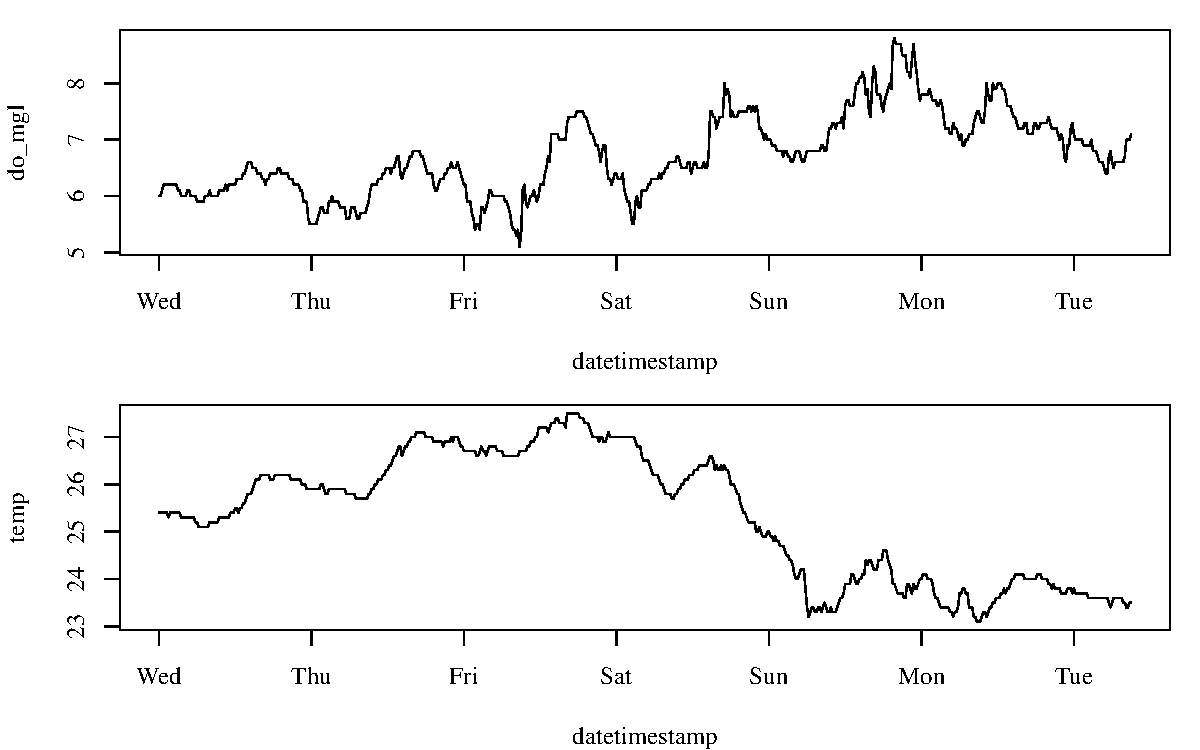
\includegraphics[width=0.7\textwidth]{figure/sub_plo} 

}



\end{knitrout}
\end{frame}

%%%%%%
\begin{frame}[containsverbatim]{Organize SWMP data}
Common problems with `subset.swmpr'...
\begin{knitrout}\scriptsize
\definecolor{shadecolor}{rgb}{0.969, 0.969, 0.969}\color{fgcolor}\begin{kframe}
\begin{alltt}
\hlcom{# incorrect subset argument format, no time}
\hlkwd{subset}\hlstd{(wq_dat,} \hlkwc{subset} \hlstd{=} \hlkwd{c}\hlstd{(}\hlstr{'2012-01-01'}\hlstd{,} \hlstr{'2012-01-31'}\hlstd{))}
\end{alltt}


{\ttfamily\noindent\bfseries\color{errorcolor}{\#\# Error: subset must be of format \%Y-\%m-\%d \%H:\%M}}\begin{alltt}
\hlcom{# forgot to include operator}
\hlkwd{subset}\hlstd{(wq_dat,} \hlkwc{subset} \hlstd{=} \hlstr{'2012-01-31 00:00'}\hlstd{)}
\end{alltt}


{\ttfamily\noindent\bfseries\color{errorcolor}{\#\# Error: Binary operator must be included if only one subset value is provided}}\begin{alltt}
\hlcom{# incorrect parameter names}
\hlkwd{subset}\hlstd{(wq_dat,} \hlkwc{select} \hlstd{=} \hlstr{'DO'}\hlstd{)}
\end{alltt}


{\ttfamily\noindent\bfseries\color{errorcolor}{\#\# Error: select argument is invalid}}\end{kframe}
\end{knitrout}
How do we fix these problems??
\end{frame}

%%%%%%
\begin{frame}[containsverbatim]{Organize SWMP data}
Now that we know how to handle QAQC flags and subset the data, what else could we do before we analyze? \\~\\
What if we want to compare time series from different datasets? \\~\\
Data are imported separately for water quality, weather, and nutrients... \\~\\
Sometimes the time step is different...\\~\\
Use the `comb.swmp' and `setstep.swmp' functions!
\begin{knitrout}\scriptsize
\definecolor{shadecolor}{rgb}{0.969, 0.969, 0.969}\color{fgcolor}\begin{kframe}
\begin{alltt}
\hlcom{# help files}
\hlopt{?}\hlstd{comb.swmpr}
\hlopt{?}\hlstd{setstep.swmpr}
\end{alltt}
\end{kframe}
\end{knitrout}
\end{frame}

%%%%%%
\begin{frame}[containsverbatim]{Organize SWMP data}
The `setstep.swmpr' function is used to standardize the time step of a swmpr object \\~\\
The `comb.swmpr' function is used to combine swmpr objects \\~\\
`setstep.swmpr' is used within `comb.swmpr' so you should not have to use it directly \\~\\
How is it done??
\end{frame}

%%%%%%
\begin{frame}[containsverbatim]{Organize SWMP data}
How can we combine SWMP data?
\begin{knitrout}\scriptsize
\definecolor{shadecolor}{rgb}{0.969, 0.969, 0.969}\color{fgcolor}\begin{kframe}
\begin{alltt}
\hlcom{# combine water quality and weather data in the same object}
\hlstd{tmp} \hlkwb{<-} \hlkwd{comb}\hlstd{(wq_dat, met_dat)}
\hlkwd{head}\hlstd{(tmp,} \hlnum{3}\hlstd{)} \hlcom{# first three rows}
\end{alltt}
\begin{verbatim}
##         datetimestamp atemp rh   bp wspd maxwspd wdir sdwdir totpar totprcp
## 1 2011-01-01 00:00:00    15 94 1019    3       3  145      8     NA       0
## 2 2011-01-01 00:15:00    15 95 1019    3       4  146      7     NA       0
## 3 2011-01-01 00:30:00    15 95 1019    3       4  139      7     NA       0
##   cumprcp totsorad temp spcond sal do_pct do_mgl depth cdepth level clevel ph
## 1       0       NA   11     44  28     68      6     2     NA    NA     NA  8
## 2       0       NA   11     44  28     68      6     2     NA    NA     NA  8
## 3       0       NA   11     44  28     68      6     2     NA    NA     NA  8
##   turb chlfluor
## 1    3       NA
## 2    3       NA
## 3    2       NA
\end{verbatim}
\end{kframe}
\end{knitrout}
\end{frame}

%%%%%%
\begin{frame}[containsverbatim]{Organize SWMP data}
What happened?  Check the attributes of the combined object...
\begin{knitrout}\scriptsize
\definecolor{shadecolor}{rgb}{0.969, 0.969, 0.969}\color{fgcolor}\begin{kframe}
\begin{alltt}
\hlcom{# attributes of combined object}

\hlcom{# stations }
\hlkwd{attr}\hlstd{(tmp,} \hlstr{'station'}\hlstd{)}
\end{alltt}
\begin{verbatim}
## [1] "apacpwq"  "apaebmet"
\end{verbatim}
\begin{alltt}
\hlcom{# date ranges, same as before}
\hlkwd{attr}\hlstd{(tmp,} \hlstr{'date_rng'}\hlstd{)}
\end{alltt}
\begin{verbatim}
## [1] "2011-01-01 00:00:00 EST" "2014-10-23 02:45:00 EST"
\end{verbatim}
\begin{alltt}
\hlcom{# parameters, both wq and met}
\hlkwd{attr}\hlstd{(tmp,} \hlstr{'parameters'}\hlstd{)}
\end{alltt}
\begin{verbatim}
##  [1] "atemp"    "rh"       "bp"       "wspd"     "maxwspd"  "wdir"    
##  [7] "sdwdir"   "totpar"   "totprcp"  "cumprcp"  "totsorad" "temp"    
## [13] "spcond"   "sal"      "do_pct"   "do_mgl"   "depth"    "cdepth"  
## [19] "level"    "clevel"   "ph"       "turb"     "chlfluor"
\end{verbatim}
\end{kframe}
\end{knitrout}
\end{frame}

%%%%%%
\begin{frame}[containsverbatim]{Organize SWMP data}
We now have a swmpr object with data from two stations, why do we want this? Easier plotting...
\begin{knitrout}\scriptsize
\definecolor{shadecolor}{rgb}{0.969, 0.969, 0.969}\color{fgcolor}\begin{kframe}
\begin{alltt}
\hlcom{# plot some combined data}

\hlcom{# subset date ranges first}
\hlstd{dates} \hlkwb{<-} \hlkwd{c}\hlstd{(}\hlstr{'2012-06-01 0:0'}\hlstd{,} \hlstr{'2012-07-31 0:0'}\hlstd{)}
\hlstd{to_plot} \hlkwb{<-} \hlkwd{subset}\hlstd{(tmp,} \hlkwc{subset} \hlstd{= dates)}

\hlcom{# plot}
\hlkwd{plot}\hlstd{(atemp} \hlopt{~} \hlstd{datetimestamp, to_plot,} \hlkwc{type} \hlstd{=} \hlstr{'l'}\hlstd{,} \hlkwc{col} \hlstd{=} \hlstr{'red'}\hlstd{,} \hlkwc{ylab} \hlstd{=} \hlstr{'Temp C'}\hlstd{)}
\hlkwd{lines}\hlstd{(to_plot}\hlopt{$}\hlstd{datetimestamp, to_plot}\hlopt{$}\hlstd{temp,} \hlkwc{col} \hlstd{=} \hlstr{'blue'}\hlstd{)}
\hlkwd{title}\hlstd{(}\hlstr{'Air (red) and water (blue) temperature'}\hlstd{)}
\end{alltt}
\end{kframe}

{\centering 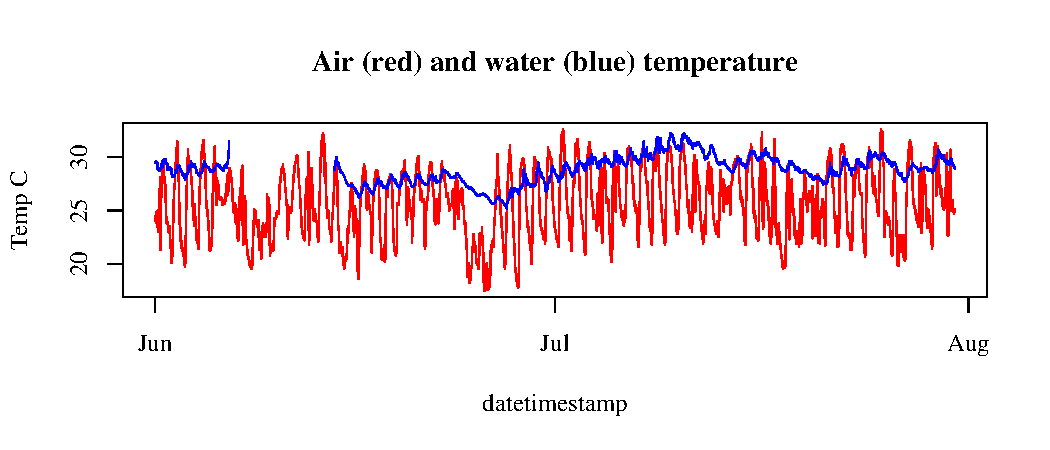
\includegraphics[width=0.7\textwidth]{figure/comb_plo} 

}



\end{knitrout}
\end{frame}

%%%%%%
\begin{frame}[containsverbatim]{Organize SWMP data}
The options for `comb.swmpr' allow flexibility \\~\\
\begin{knitrout}\scriptsize
\definecolor{shadecolor}{rgb}{0.969, 0.969, 0.969}\color{fgcolor}\begin{kframe}
\begin{alltt}
\hlcom{# arguments for the function, or ?comb.swmpr}
\hlkwd{formals}\hlstd{(comb.swmpr)}
\end{alltt}
\begin{verbatim}
## $...
## 
## 
## $timestep
## [1] 15
## 
## $differ
## [1] 5
## 
## $method
## [1] "union"
\end{verbatim}
\end{kframe}
\end{knitrout}
\end{frame}

%%%%%%
\begin{frame}[containsverbatim]{Organize SWMP data}
What do the arguments specify? \\~\\
\begin{itemize}
\item ... : input swmpr data, separated by comma\\~\\
\item timestep: minutes defining the standardized time step\\~\\
\item differ: maximum difference in minutes for matching observations with original time steps to standardized time steps \\`\\
\item method: how the data are combined using the time stamps - union, intersect, or using a station
\end{itemize}
\end{frame}

%%%%%%
\begin{frame}[containsverbatim]{Organize SWMP data}
Changing the `timestep' argument can be useful for reducing data volume...
\begin{knitrout}\scriptsize
\definecolor{shadecolor}{rgb}{0.969, 0.969, 0.969}\color{fgcolor}\begin{kframe}
\begin{alltt}
\hlcom{# dimension of earlier combined object}
\hlkwd{dim}\hlstd{(tmp)}
\end{alltt}
\begin{verbatim}
## [1] 133548     24
\end{verbatim}
\begin{alltt}
\hlcom{# create new object at two hour time step}
\hlstd{tmp} \hlkwb{<-} \hlkwd{comb}\hlstd{(wq_dat, met_dat,} \hlkwc{timestep} \hlstd{=} \hlnum{120}\hlstd{)}
\hlkwd{dim}\hlstd{(tmp)}
\end{alltt}
\begin{verbatim}
## [1] 16695    24
\end{verbatim}
\end{kframe}
\end{knitrout}
\end{frame}

%%%%%%
\begin{frame}[containsverbatim]{Organize SWMP data}
Changing the `timestep' argument can be useful for reducing data volume...
\begin{knitrout}\scriptsize
\definecolor{shadecolor}{rgb}{0.969, 0.969, 0.969}\color{fgcolor}\begin{kframe}
\begin{alltt}
\hlcom{# note the time step in datetimestamp}
\hlkwd{head}\hlstd{(tmp,} \hlnum{4}\hlstd{)}
\end{alltt}
\begin{verbatim}
##         datetimestamp atemp rh   bp wspd maxwspd wdir sdwdir totpar totprcp
## 1 2010-12-31 23:00:00    NA NA   NA   NA      NA   NA     NA     NA      NA
## 2 2011-01-01 01:00:00    15 95 1018    3       4  144      6     NA       0
## 3 2011-01-01 03:00:00    15 93 1017    6       7  137      7     NA       0
## 4 2011-01-01 05:00:00    15 95 1017    4       6  146      8     NA       0
##   cumprcp totsorad temp spcond sal do_pct do_mgl depth cdepth level clevel ph
## 1      NA       NA   NA     NA  NA     NA     NA    NA     NA    NA     NA NA
## 2       0       NA   11     44  29     68      6     2     NA    NA     NA  8
## 3       0       NA   11     45  29     66      6     2     NA    NA     NA  8
## 4       0       NA   11     44  28     66      6     1     NA    NA     NA  8
##   turb chlfluor
## 1   NA       NA
## 2    2       NA
## 3    3       NA
## 4    2       NA
\end{verbatim}
\end{kframe}
\end{knitrout}
\end{frame}

%%%%%%
\begin{frame}[containsverbatim]{Organize SWMP data}
\alert{Caution!} Standardizing a time series to a set time step may impose some inaccuracy \\~\\
Observations are matched as close in time as possible to the standardized time series \\~\\
For example, if we set the time step at 60 minute intervals and actual observations are taken every 15 and 45 minutes of the hour \\~\\
Which observations are matched and which are discarded? \\~\\
By default, `comb.swmpr' matches the closest observation and discards the rest \\~\\
`Close' is defined by the `differ' argument
\end{frame}

%%%%%%
\begin{frame}[containsverbatim]{Organize SWMP data}
The `differ' argument defines the maximum time difference for matching observations to the standardized time step \\~\\
The maximum allowed value for `differ' is one half the time step -- values beyond this window will create duplicates in your data \\~\\
For example, set a 60 minute time step -- 5pm, 6pm, 7pm, etc., consider an observation at 635pm \\~\\
\begin{columns}[T]
\begin{column}{0.45\textwidth}
\alert{wrong!}\\
\begin{itemize}
\item `differ' is 40 minutes
\item observation will be duplicated at 6pm and 7pm \\~\\
\end{itemize}
\end{column}
\begin{column}{0.45\textwidth}
\alert{right!}
\begin{itemize}
\item `differ' is 30 minutes
\item observation is matched only to 7pm \\~\\
\end{itemize}
\end{column}
\end{columns}
Again, default behavior of `comb.swmpr' prevents duplication
\end{frame}

%%%%%%
\begin{frame}[containsverbatim]{Organize SWMP data}
Consider the alternative scenario of a using a conservative value for `differ'\\~\\
For example, set a 60 minute time step -- 5pm, 6pm, 7pm, etc., consider an observation at 635pm\\~\\
If `differ' is five minutes, there will be no data in the standardized time series! \\~\\
Fortunately, most SWMP data already follow a standard 15 minute time step
\begin{knitrout}\scriptsize
\definecolor{shadecolor}{rgb}{0.969, 0.969, 0.969}\color{fgcolor}\begin{kframe}
\begin{alltt}
\hlcom{# note the pre-existing time steps}
\hlkwd{head}\hlstd{(wq_dat}\hlopt{$}\hlstd{datetimestamp)}
\end{alltt}
\begin{verbatim}
## [1] "2011-01-01 00:00:00 EST" "2011-01-01 00:15:00 EST"
## [3] "2011-01-01 00:30:00 EST" "2011-01-01 00:45:00 EST"
## [5] "2011-01-01 01:00:00 EST" "2011-01-01 01:15:00 EST"
\end{verbatim}
\end{kframe}
\end{knitrout}
\end{frame}

%%%%%%
\begin{frame}[containsverbatim]{Organize SWMP data}
However, nutrient data may have irregular time stamps since these data are not from `continuous' monitoring station 
\begin{knitrout}\scriptsize
\definecolor{shadecolor}{rgb}{0.969, 0.969, 0.969}\color{fgcolor}\begin{kframe}
\begin{alltt}
\hlcom{# note irregular time stamps on nutrient data}
\hlkwd{head}\hlstd{(nut_dat)}
\end{alltt}
\begin{verbatim}
##         datetimestamp  po4f nh4f no2f no3f no23f chla_n
## 1 2011-01-11 11:28:00    NA 0.04   NA   NA    NA      4
## 2 2011-02-09 12:51:00 0.005   NA   NA   NA  0.09      8
## 3 2011-02-09 12:55:00 0.004   NA   NA   NA  0.10      9
## 4 2011-02-09 13:03:00 0.004   NA   NA   NA  0.07      8
## 5 2011-03-02 10:36:00 0.004   NA   NA   NA  0.05      5
## 6 2011-04-06 11:29:00    NA 0.04   NA   NA  0.24      9
\end{verbatim}
\end{kframe}
\end{knitrout}
Use caution if combining these data or standardizing the time step - there is potential for data omission or extrapolation
\end{frame}

%%%%%%
\begin{frame}[containsverbatim]{Organize SWMP data}
Case in point, try standardizing the nutrient time series with `setstep.swmpr'
\begin{knitrout}\scriptsize
\definecolor{shadecolor}{rgb}{0.969, 0.969, 0.969}\color{fgcolor}\begin{kframe}
\begin{alltt}
\hlkwd{dim}\hlstd{(nut_dat)} \hlcom{# initial dimensions}
\end{alltt}
\begin{verbatim}
## [1] 48  7
\end{verbatim}
\begin{alltt}
\hlcom{# standardize nutrient time series}
\hlstd{tmp} \hlkwb{<-} \hlkwd{setstep}\hlstd{(nut_dat,} \hlkwc{timestep} \hlstd{=} \hlnum{60}\hlstd{,} \hlkwc{differ} \hlstd{=} \hlnum{5}\hlstd{)}
\hlkwd{dim}\hlstd{(tmp)}
\end{alltt}
\begin{verbatim}
## [1] 25369     7
\end{verbatim}
\begin{alltt}
\hlcom{# remove empty rows, columns}
\hlstd{tmp} \hlkwb{<-} \hlkwd{subset}\hlstd{(tmp,} \hlkwc{rem_row} \hlstd{= T,} \hlkwc{rem_col} \hlstd{= T)}
\hlstd{tmp} \hlcom{#only four rows!}
\end{alltt}
\begin{verbatim}
##         datetimestamp  po4f nh4f no23f chla_n
## 1 2011-02-09 13:00:00 0.004   NA 0.075      8
## 2 2012-07-03 10:00:00 0.004 0.07 0.057      6
## 3 2012-09-05 11:00:00    NA 0.03 0.007      9
## 4 2013-07-09 09:00:00 0.004 0.06 0.036      7
\end{verbatim}
\end{kframe}
\end{knitrout}
\end{frame}

%%%%%%
\begin{frame}[containsverbatim]{Organize SWMP data}
A final note about combining data... what about combining data with different \alert{time ranges}\\~\\
Consider combining two datasets \\~\\
\begin{itemize}
\item \alert{Scenario 1}: Time ranges are the same
\item \alert{Scenario 2}: Time ranges are not the same, but there is overlap
\item \alert{Scenario 3}: Time ranges are not the same, there is no overlap \\~\\
\end{itemize}
The `method' argument of `comb.swmpr' allows flexibility under different scenarios - time range intersect, union, or range of one station
\end{frame}

%%%%%%
\begin{frame}{Organize SWMP data}
\onslide<+->
\alert{Scenario 1}: Time ranges are the same \\~\\
Don't worry about changing the `method' argument - it will have no effect\\~\\
Our previous examples represent scenario 1 \\~\\
\onslide<+->
\alert{Scenario 2}: Time ranges are not the same, but there is overlap \\~\\
\begin{itemize}
\item union: the default method, use the whole time range of both datasets
\item intersect: use only the time range that is shared between the two
\item or enter one of the station names, this says use the time range belonging to that station\\~\\
\end{itemize}
\onslide<+->
\alert{Scenario 3}: Time ranges are not the same, there is no overlap \\~\\
The only method that makes sense is `union'
\end{frame}

%%%%%%
\begin{frame}[containsverbatim]{Organize SWMP data}
Try some examples
\begin{knitrout}\scriptsize
\definecolor{shadecolor}{rgb}{0.969, 0.969, 0.969}\color{fgcolor}\begin{kframe}
\begin{alltt}
\hlcom{# first we subset for the example}
\hlstd{sub1} \hlkwb{<-} \hlkwd{subset}\hlstd{(wq_dat,} \hlkwc{subset} \hlstd{=} \hlkwd{c}\hlstd{(}\hlstr{'2012-07-01 0:0'}\hlstd{,} \hlstr{'2012-07-31 0:0'}\hlstd{))}
\hlstd{sub2} \hlkwb{<-} \hlkwd{subset}\hlstd{(met_dat,} \hlkwc{subset} \hlstd{=} \hlkwd{c}\hlstd{(}\hlstr{'2012-07-15 0:0'}\hlstd{,} \hlstr{'2012-08-12 0:0'}\hlstd{))}

\hlcom{# what are the date ranges?}
\hlkwd{attr}\hlstd{(sub1,} \hlstr{'date_rng'}\hlstd{)}
\end{alltt}
\begin{verbatim}
## [1] "2012-07-01 EST" "2012-07-31 EST"
\end{verbatim}
\begin{alltt}
\hlkwd{attr}\hlstd{(sub2,} \hlstr{'date_rng'}\hlstd{)}
\end{alltt}
\begin{verbatim}
## [1] "2012-07-15 EST" "2012-08-12 EST"
\end{verbatim}
\end{kframe}
\end{knitrout}
\end{frame}

%%%%%%
\begin{frame}[containsverbatim]{Organize SWMP data}
Try some examples
\begin{knitrout}\scriptsize
\definecolor{shadecolor}{rgb}{0.969, 0.969, 0.969}\color{fgcolor}\begin{kframe}
\begin{alltt}
\hlcom{# combine using union, this is the default}
\hlstd{tmp} \hlkwb{<-} \hlkwd{comb}\hlstd{(sub1, sub2,} \hlkwc{method} \hlstd{=} \hlstr{'union'}\hlstd{)}

\hlcom{# what is the date range of the combined object?}
\hlkwd{attr}\hlstd{(tmp,} \hlstr{'date_rng'}\hlstd{)}
\end{alltt}
\begin{verbatim}
## [1] "2012-07-01 EST" "2012-08-12 EST"
\end{verbatim}
\end{kframe}
\end{knitrout}
\end{frame}

%%%%%%
\begin{frame}[containsverbatim]{Organize SWMP data}
Try some examples
\begin{knitrout}\scriptsize
\definecolor{shadecolor}{rgb}{0.969, 0.969, 0.969}\color{fgcolor}\begin{kframe}
\begin{alltt}
\hlcom{# combine using intersect}
\hlstd{tmp} \hlkwb{<-} \hlkwd{comb}\hlstd{(sub1, sub2,} \hlkwc{method} \hlstd{=} \hlstr{'intersect'}\hlstd{)}

\hlcom{# what is the date range of the combined object?}
\hlkwd{attr}\hlstd{(tmp,} \hlstr{'date_rng'}\hlstd{)}
\end{alltt}
\begin{verbatim}
## [1] "2012-07-15 EST" "2012-07-31 EST"
\end{verbatim}
\end{kframe}
\end{knitrout}
\end{frame}

%%%%%%
\begin{frame}[containsverbatim]{Organize SWMP data}
Try some examples
\begin{knitrout}\scriptsize
\definecolor{shadecolor}{rgb}{0.969, 0.969, 0.969}\color{fgcolor}\begin{kframe}
\begin{alltt}
\hlcom{# combine using the time range in sub1}
\hlstd{station} \hlkwb{<-} \hlkwd{attr}\hlstd{(sub1,} \hlstr{'station'}\hlstd{)}
\hlstd{tmp} \hlkwb{<-} \hlkwd{comb}\hlstd{(sub1, sub2,} \hlkwc{method} \hlstd{= station)}

\hlcom{# what is the date range of the combined object?}
\hlkwd{attr}\hlstd{(tmp,} \hlstr{'date_rng'}\hlstd{)}
\end{alltt}
\begin{verbatim}
## [1] "2012-07-01 EST" "2012-07-31 EST"
\end{verbatim}
\end{kframe}
\end{knitrout}
\end{frame}

%%%%%%
\begin{frame}[containsverbatim]{Organize SWMP data}
Now you have an idea of how to organize SWMP data for analysis!\\~\\
Here's what we did:\\~\\
\begin{itemize}
\item Evaluate QAQC flags in the data and handle accordingly \\~\\
\item Subsetting the data to remove empty rows/columns or to select variables or time ranges of interest \\~\\
\item Combining data for comparison or data simplification \\~\\
\end{itemize}
Consult the SWMPr cookboook for an example workflow! \\~\\
After lunch... what are some basic ways we can analyze the data?
\end{frame}

%%%%%%
\begin{frame}
\vspace{0.3in}
\centerline{
\begin{tikzpicture}
  \node[drop shadow={shadow xshift=0ex,shadow yshift=0ex},fill=white,draw] at (0,0) {
\includegraphics[width=0.9\textwidth]{bg_main.jpg}};
\end{tikzpicture}}
\vspace{0.5in}
\Large
\centerline{\Bigtxt{Questions??}}
\end{frame}

\end{document}
